\documentclass[tikz]{standalone}
\usepackage{pgfplots}
\pgfplotsset{compat=1.15}
\usepackage{mathrsfs}
\usetikzlibrary{arrows,calc}
\usepackage{tkz-euclide}

\pagestyle{empty}

\definecolor{AngleClr}{rgb}{0,0.39215686274509803,0}
\definecolor{ShapeClr}{rgb}{0.6,0.2,0}

\begin{document}

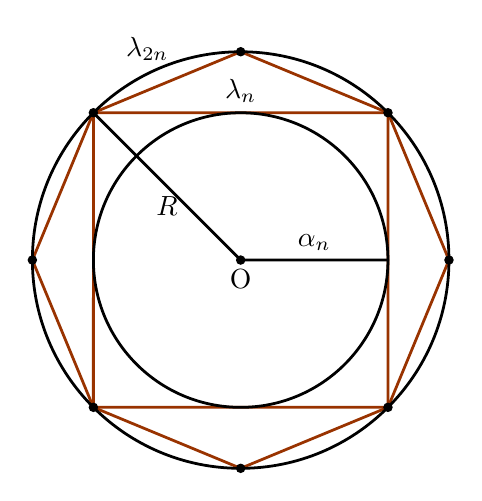
\begin{tikzpicture}[scale=.75]
\tkzSetUpLine[line width=1pt,color=black]
\tkzSetUpPoint[fill=black]

\tkzDefPoints{0/0/P0}
\tkzDefPoint(22.5:2.7){P1}

\tkzDefRegPolygon[side,sides=8](P0,P1)

\tkzDefCircle[circum](P1,P2,P3) \tkzGetPoint{O}
\tkzInterLL(O,P3)(P4,P2) \tkzGetPoint{M}

\tkzFillPolygon[fill=white](P1,P2,P3,P4,P5,P6,P7,P8)

\tkzDrawPolygon[color=ShapeClr](P1,P2,P3,P4,P5,P6,P7,P8)
\tkzDrawPolygon[color=ShapeClr](P2,P4,P6,P8)

\tkzDrawCircle[line width=1pt,black](O,P1)
\tkzDrawSegments(O,P6 O,M)

\tkzDrawCircle[line width=1pt,black](O,M)
\tkzLabelSegment(O,P6){$R$}
\tkzLabelSegment[above](P4,P6){$\lambda_n$}
\tkzLabelSegment[yshift=0.7cm,xshift=-0.25cm](P6,P5){$\lambda_{2n}$}
\tkzLabelSegment[above](O,M){$\alpha_n$}

\tkzDrawPoints[size=3](P1,P2,P3,P4,P5,P6,P7,P8,O)

\tkzLabelPoint[below](O){$\rm O$}

\end{tikzpicture}

\end{document}
